%!Mode:: "TeX:UTF-8"
% !TEX program  = xelatex
\documentclass[a4paper,11pt,UTF8,AutoFakeBold]{ctexart}

% 引入宏定义 macros.tex
% !TeX program = xelatex

\usepackage{indentfirst} %缩进
\usepackage{xeCJK}    %使用系统字体
\usepackage{bm}       %粗体
\usepackage{fancyhdr} %自定义页眉页脚
%\pagestyle{empty}    % 没有页眉页脚
\pagestyle{plain}     % 没有页眉,页脚包含一个居中的页码
\usepackage{amsmath, amsthm, amssymb, amsfonts} %数学公式
\usepackage[a4paper,left=3cm,right=3cm,top=3.5cm,bottom=3.5cm]{geometry}
\usepackage{booktabs} %插入表格
\usepackage[section]{placeins} %避免浮动
\usepackage{listings} %插入代码
\usepackage{underscore} % 在非数学环境下不再需要转义 '_'
\usepackage{ctex}     %中文宏包
\usepackage[svgnames, table]{xcolor} %彩色表格
\usepackage{algorithm}          %伪代码
\usepackage{algorithmicx}
\usepackage{algpseudocode}
\usepackage{algorithm,algpseudocode,float}
\usepackage{lipsum}
\usepackage{enumitem}           %调整列举环境
\usepackage{url}
\usepackage{fontspec,xunicode}
\usepackage{tabularx}            % 增强表格
\usepackage{multirow}            % 多行、多列
\defaultfontfeatures{Mapping=tex-text} %如果没有它,会有一些 tex 特殊字符无法正常使用,比如连字符。
\usepackage[explicit]{titlesec}
\usepackage[breaklinks,colorlinks,linkcolor=black,citecolor=black,urlcolor=black]{hyperref} % 生成 PDF 书签
\usepackage{float}
\usepackage{xifthen} % provides \isempty test



\usepackage{graphicx}
\graphicspath{{imgs/}}

%%%%%%%%%%%%%%%%%%%%%%%%%%%%%%%%%%%%%%%%%%%%%%%%%%%%%%%%%%%%%%%%
% 缩进及行间距
%%%%%%%%%%%%%%%%%%%%%%%%%%%%%%%%%%%%%%%%%%%%%%%%%%%%%%%%%%%%%%%%
\setlength{\parindent}{22bp} %重新定义缩进长度
\linespread{1}

%%%%%%%%%%%%%%%%%%%%%%%%%%%%%%%%%%%%%%%%%%%%%%%%%%%%%%%%%%%%%%%%
% 图的标题行间距设置
%%%%%%%%%%%%%%%%%%%%%%%%%%%%%%%%%%%%%%%%%%%%%%%%%%%%%%%%%%%%%%%%
\newcommand{\bottomcaption}{%
    \setlength{\abovecaptionskip}{6bp}%
    \setlength{\belowcaptionskip}{6bp}%
    \caption
}

%%%%%%%%%%%%%%%%%%%%%%%%%%%%%%%%%%%%%%%%%%%%%%%%%%%%%%%%%%%%%%%%
% 字体定义
%%%%%%%%%%%%%%%%%%%%%%%%%%%%%%%%%%%%%%%%%%%%%%%%%%%%%%%%%%%%%%%%
\setmainfont{Times New Roman}  %默认英文字体.serif是有衬线字体sans serif无衬线字体
\setmonofont{Consolas}
\setCJKmainfont[ItalicFont={宋体}, BoldFont={黑体}]{宋体}%衬线字体 缺省中文字体为 
% \punctstyle{hangmobanjiao}
%-----------------------xeCJK下设置中文字体------------------------------%
\setCJKfamilyfont{song}{SimSun}                             %宋体 song
\newcommand{\song}{\CJKfamily{song}}
\setCJKfamilyfont{fs}{FangSong}                      %仿宋  fs
\newcommand{\fs}{\CJKfamily{fs}}
\let\kaishu\relax                                    %重定义楷体,打开假粗体
\newCJKfontfamily\kaishu{KaiTi}[AutoFakeBold]
%\setCJKfamilyfont{ktgb}{KaiTi_GB2312}                      %楷体 GB2312
%\newcommand{\ktgb}{\CJKfamily{ktgb}}
\setCJKfamilyfont{yh}{Microsoft YaHei}                    %微软雅黑 yh
\newcommand{\yh}{\CJKfamily{yh}}
\setCJKfamilyfont{hei}{SimHei}                              %黑体  hei
\newcommand{\hei}{\CJKfamily{hei}}
\setCJKfamilyfont{hwxk}{STXingkai}                                %华文行楷  hwxk
\newcommand{\hwxk}{\CJKfamily{hwxk}}
\setCJKfamilyfont{fzshu}{FZShuTi}                                    %方正舒体 fzshu
\newcommand{\fzshu}{\CJKfamily{fzshu}}
%------------------------------设置字体大小------------------------%
\newcommand{\chuhao}{\fontsize{42bp}{63bp}\selectfont}     %初号, 1.5倍行距
\newcommand{\xiaochuhao}{\fontsize{36bp}{36bp}\selectfont} %小初号,单倍行距
\newcommand{\yihao}{\fontsize{26bp}{39bp}\selectfont}        % 一号, 1.5 倍行距
\newcommand{\erhao}{\fontsize{22bp}{33bp}\selectfont}        % 二号, 1.5倍行距
\newcommand{\xiaoerhao}{\fontsize{18bp}{18bp}\selectfont}       % 小二, 单倍行距
\newcommand{\sanhao}{\fontsize{16bp}{24bp}\selectfont}       % 三号, 1.5倍行距
\newcommand{\xiaosanhao}{\fontsize{15bp}{22bp}\selectfont}      % 小三, 1.5倍行距
\newcommand{\sihao}{\fontsize{14bp}{21bp}\selectfont}        % 四号, 1.5 倍行距
\newcommand{\banxiaosi}{\fontsize{13bp}{20bp}\selectfont}  % 半小四, 20pt行距
\newcommand{\xiaosihao}{\fontsize{12bp}{20bp}\selectfont}       % 小四, 20pt行距
\newcommand{\dawuhao}{\fontsize{11bp}{11bp}\selectfont}      % 大五号, 单倍行距
\newcommand{\wuhao}{\fontsize{10.5bp}{10.5bp}\selectfont}   % 五号, 单倍行距
\newcommand{\xiaowuhao}{\fontsize{9bp}{9bp}\selectfont}   %小五号,单倍行距
%------------------------------重定义normalize------------------------%
\renewcommand{\normalsize}{\fontsize{12bp}{20bp}\selectfont}


%%%%%%%%%%%%%%%%%%%%%%%%%%%%%%%%%%%%%%%%%%%%%%%%%%%%%%%%%%%%%%%%
% 图题字体大小相同
%%%%%%%%%%%%%%%%%%%%%%%%%%%%%%%%%%%%%%%%%%%%%%%%%%%%%%%%%%%%%%%%
\usepackage{caption}
\captionsetup{font={footnotesize}}   % footnotesize = 9bp
\captionsetup[lstlisting]{font={footnotesize}}

%%%%%%%%%%%%%%%%%%%%%%%%%%%%%%%%%%%%%%%%%%%%%%%%%%%%%%%%%%%%%%%%
% 重定义枚举编号为 1),2)...
%%%%%%%%%%%%%%%%%%%%%%%%%%%%%%%%%%%%%%%%%%%%%%%%%%%%%%%%%%%%%%%%
\renewcommand{\labelenumi}{\theenumi)}


%%%%%%%%%%%%%%%%%%%%%%%%%%%%%%%%%%%%%%%%%%%%%%%%%%%%%%%%%%%%%%%%
% 重定义section标题
%%%%%%%%%%%%%%%%%%%%%%%%%%%%%%%%%%%%%%%%%%%%%%%%%%%%%%%%%%%%%%%%
\CTEXsetup[format={\song\bfseries\zihao{4}},number={\chinese{section}},name={,、~},aftername={},indent={0bp},beforeskip={6bp},afterskip={6bp},format+={\flushleft}]{section}
\CTEXsetup[format={\Large\bfseries\song\zihao{5}},name={(,)},number={\chinese{subsection}},aftername={},indent={22bp},beforeskip={6bp},afterskip={6bp}]{subsection}
\CTEXsetup[format={\Large\bfseries\song\zihao{5}},name={,.},aftername={ },indent={28bp},beforeskip={6bp},afterskip={6bp}]{subsubsection}
\CTEXsetup[number={\chinese{section}},name={附录, ~~ }]{appendix}



%%%%%%%%%%%%%%%%%%%%%%%%%%%%%%%%%%%%%%%%%%%%%%%%%%%%%%%%%%%%%%%%
% 标题名称中文化
%%%%%%%%%%%%%%%%%%%%%%%%%%%%%%%%%%%%%%%%%%%%%%%%%%%%%%%%%%%%%%%%
\renewcommand\figurename{\hei 图}
\renewcommand\tablename{\hei 表}
\renewcommand\lstlistingname{\hei 代码}
\renewcommand{\algorithmicrequire}{\textbf{输入:}}
\renewcommand{\algorithmicensure}{\textbf{输出:}}
\newtheorem{define}{定义}


%%%%%%%%%%%%%%%%%%%%%%%%%%%%%%%%%%%%%%%%%%%%%%%%%%%%%%%%%%%%%%%%
% 列表设置
%%%%%%%%%%%%%%%%%%%%%%%%%%%%%%%%%%%%%%%%%%%%%%%%%%%%%%%%%%%%%%%%
\setlist[enumerate,1]{leftmargin=46bp,listparindent=0bp,itemsep=0mm,partopsep=.7mm,parsep=0ex,labelsep=1.5mm,topsep=0.7mm}
\setlist[enumerate,2]{label=\alph*),leftmargin=1.5em}  %二级item设置
\setitemize{leftmargin=46bp,listparindent=0bp,itemsep=0mm,partopsep=.7mm,parsep=0ex,labelsep=1.5mm,topsep=0.7mm}
\setitemize{itemindent=38bp,leftmargin=0bp,itemsep=-0.4ex,listparindent=26bp,partopsep=0bp,parsep=0.5ex,topsep=-0.25ex}
%\setdescription{itemindent=38bp,leftmargin=0bp,itemsep=-0.4ex,listparindent=26bp,partopsep=0bp,parsep=0.5ex,topsep=-0.25ex}

%%%%%%%%%%%%%%%%%%%%%%%%%%%%%%%%%%%%%%%%%%%%%%%%%%%%%%%%%%%%%%%%
% 代码设置
%%%%%%%%%%%%%%%%%%%%%%%%%%%%%%%%%%%%%%%%%%%%%%%%%%%%%%%%%%%%%%%%
\lstset{
 columns=fixed,
 numbers=left,                                        % 在左侧显示行号
 numberstyle=\tiny\color{gray},                       % 设定行号格式
 frame=single,                                        % 单线背景边框
 breaklines=true,                                     % 设定LaTeX对过长的代码行进行自动换行
 keywordstyle=\color[RGB]{40,40,255},                 % 设定关键字颜色
 numberstyle=\footnotesize\color{darkgray},
 commentstyle=\it\color[RGB]{0,96,96},                % 设置代码注释的格式
 stringstyle=\rmfamily\slshape\color[RGB]{128,0,0},   % 设置字符串格式
 showstringspaces=false,                              % 不显示字符串中的空格
 language=java,                                        % 设置语言
 basicstyle=\linespread{1.0}\xiaowuhao\ttfamily,                      % 字体字号
 %lineskip=10bp,
 %baselinestretch=1,
}


%%%%%%%%%%%%%%%%%%%%%%%%%%%%%%%%%%%%%%%%%%%%%%%%%%%%%%%%%%%%%%%%
% 伪代码分页
%%%%%%%%%%%%%%%%%%%%%%%%%%%%%%%%%%%%%%%%%%%%%%%%%%%%%%%%%%%%%%%%
\makeatletter
\renewcommand{\ALG@name}{算法}
\newenvironment{breakablealgorithm}
  {% \begin{breakablealgorithm}
   \begin{center}
     \refstepcounter{algorithm}% New algorithm
     \hrule height.8bp depth0bp \kern2bp% \@fs@pre for \@fs@ruled
     \renewcommand{\caption}[2][\relax]{% Make a new \caption
       {\raggedright\textbf{\ALG@name~\thealgorithm} ##2\par}%
       \ifx\relax##1\relax % #1 is \relax
         \addcontentsline{loa}{algorithm}{\protect\numberline{\thealgorithm}##2}%
       \else % #1 is not \relax
         \addcontentsline{loa}{algorithm}{\protect\numberline{\thealgorithm}##1}%
       \fi
       \kern2bp\hrule\kern2bp
     }
  }{% \end{breakablealgorithm}
     \kern2bp\hrule\relax% \@fs@post for \@fs@ruled
   \end{center}
  }
\makeatother


%%%%%%%%%%%%%%%%%%%%%%%%%%%%%%%%%%%%%%%%%%%%%%%%%%%%%%%%%%%%%%%%
% 设置 \part
%%%%%%%%%%%%%%%%%%%%%%%%%%%%%%%%%%%%%%%%%%%%%%%%%%%%%%%%%%%%%%%%

\titleformat{\part}[display]{}{}{0pt}{}
%\titlespacing*{\part}{0pt}{0pt}{0pt}   % 在正文中隐藏 part
\makeatletter
\@addtoreset{section}{part} % 使 section 在 part 后重新标号
\makeatother


%%%%%%%%%%%%%%%%%%%%%%%%%%%%%%%%%%%%%%%%%%%%%%%%%%%%%%%%%%%%%%%%
% 设置个人信息
%%%%%%%%%%%%%%%%%%%%%%%%%%%%%%%%%%%%%%%%%%%%%%%%%%%%%%%%%%%%%%%%
\makeatletter
\newcommand{\course}[1]{
    \newcommand{\report@course}{#1}
}
\newcommand{\college}[1]{
    \newcommand{\report@college}{#1}
}
\newcommand{\major}[1]{
    \newcommand{\report@major}{#1}
}
\newcommand{\studentid}[1]{
    \newcommand{\report@studentid}{#1}
}
%\newcommand{\theauthor}[1]{
%    \newcommand{\report@author}{#1}
%}
\newcommand{\teacher}[1]{
    \newcommand{\report@teacher}{#1}
}
\newcommand{\thedate}[1]{
    \newcommand{\report@date}{#1}
}
\makeatother


%%%%%%%%%%%%%%%%%%%%%%%%%%%%%%%%%%%%%%%%%%%%%%%%%%%%%%%%%%%%%%%%
% 设置 \maketitle
%%%%%%%%%%%%%%%%%%%%%%%%%%%%%%%%%%%%%%%%%%%%%%%%%%%%%%%%%%%%%%%%
\makeatletter
\renewcommand{\maketitle}{
    \thispagestyle{empty}   % 去掉首页页码
    \begin{titlepage}

        \begin{figure}[!htbp]
            \centering
            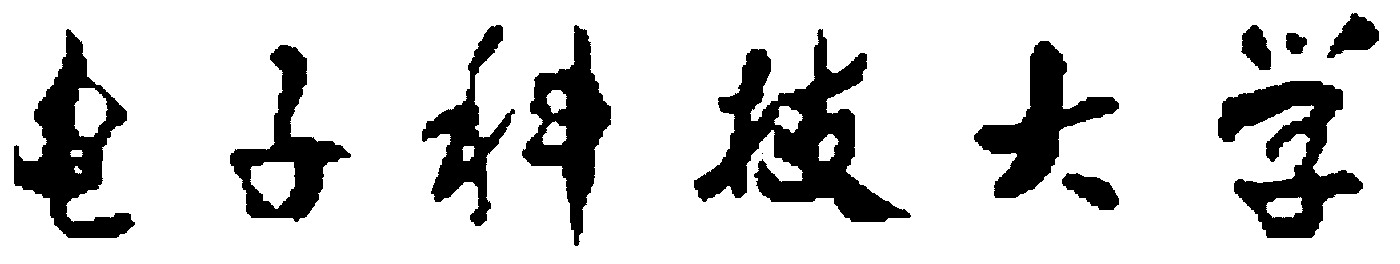
\includegraphics[width=\textwidth]{uestc}
        \end{figure}

        \center{\xiaochuhao{\kaishu 计算机专业类课程}}
        \vspace{1.5cm}
        \center{\fontsize{48bp}{52bp}{\song{\bfseries 实\\验\\报\\告}}}

        \vspace{1.5cm}

        \begin{center}
            \begin{large}
                \begin{tabular}{rl}
                    \xiaoerhao{\bfseries\fs{课程名称:}}& \xiaoerhao{\bfseries\hei{\report@course}}\\
                    \\
                    \xiaoerhao{\bfseries\fs{学\qquad 院:}}& \xiaoerhao{\bfseries\hei{\report@college}}\\
                    \\
                    \xiaoerhao{\bfseries\fs{学院专业:}}& \xiaoerhao{\bfseries\hei{\report@major}}\\
                    \\
                    \xiaoerhao{\bfseries\fs{学\qquad 号:}}& \xiaoerhao{\bfseries\hei{\report@studentid}}\\
                    \\
                    \xiaoerhao{\bfseries\fs{学生姓名:}}& \xiaoerhao{\bfseries\hei{\@author}}\\
                    \\
                    \xiaoerhao{\bfseries\fs{指导教师:}}& \xiaoerhao{\bfseries\hei{\report@teacher}}\\
                    \\
                    \xiaoerhao{\bfseries\fs{日\qquad 期:}}& \xiaoerhao{\bfseries\hei{\report@date}}\\
                \end{tabular}
            \end{large}
        \end{center}
    \end{titlepage}
    \newpage
    \setcounter{page}{1} % 第二页从 1 开始标号
}
\makeatother

%%%%%%%%%%%%%%%%%%%%%%%%%%%%%%%%%%%%%%%%%%%%%%%%%%%%%%%%%%%%%%%%
% 设置 \chapter
%%%%%%%%%%%%%%%%%%%%%%%%%%%%%%%%%%%%%%%%%%%%%%%%%%%%%%%%%%%%%%%%

\makeatletter
\newcommand{\chapter}[3]{
    \newpage
    \part{}
    \vspace*{-120bp} % Adjust the vertical space here
    \centerline{\\[40bp]\erhao{\fzshu{\bfseries 电 ~子 ~科~ 技~ 大~ 学}}}
    \vspace*{-20bp} % Adjust the vertical space her
    \centerline{\\[20bp]\yihao{\hei{\bfseries 实  ~~~ 验  ~~~ 报  ~~~ 告}}}

    \ifthenelse{\isempty{#3}}{
        \centerline{\\[20bp]\yihao{\song{\bfseries #1}}}
    }{
        \noindent
        \begin{tabularx}{\textwidth}{XXX}
            \Large\bfseries\song\zihao{4}学生姓名:{\@author} &
            \Large\bfseries\song\zihao{4}学 号:{\report@studentid} &
            \Large\bfseries\song\zihao{4}指导教师:{\report@teacher}
        \end{tabularx}\\

        \noindent
        \begin{tabularx}{\textwidth}{XX}
            \Large\bfseries\song\zihao{4}实验地点:{#2} &
            \Large\bfseries\song\zihao{4}实验时间:{#3}
        \end{tabularx}
    }
}
\makeatother



\begin{document}
\xiaosihao \setCJKfamilyfont{song}{SimSun}  

\course{计算机视觉与模式识别}
\college{计算机科学与工程学院}
\major{计算机科学与技术}
\studentid{2022010910017}
\author{谢卿云}
\teacher{沈复民}
\thedate{2025 年 5 月 10 日}

% \maketitle

%\chapter{实验一}{}{}                                      % 用于单次实验报告开头的 “实验X”
\chapter{}{}{}           % 实验信息

\section{实验项目名称:}
Scene Recognition with Bag of Words

\section{实验原理:}
\subsection{目标检测概述}
目标检测是计算机视觉领域的一个重要分支,
旨在识别图像或视频中特定目标的位置和类别。
它结合了图像分类和目标定位两项任务,
是许多高级视觉应用(如自动驾驶、智能监控、机器人视觉等)的基础。

\subsection{目标检测算法分类}
目标检测算法大致可以分为两类:
\begin{itemize}
    \item \textbf{两阶段检测器 (Two-stage Detectors)}:
    这类算法首先生成候选区域(Region Proposals),
    然后对这些候选区域进行分类和边界框回归。
    代表算法有R-CNN系列(R-CNN, Fast R-CNN, Faster R-CNN)。
    \item \textbf{单阶段检测器 (One-stage Detectors)}:
    这类算法直接在图像上预测目标的类别和边界框,
    无需生成候选区域。代表算法有YOLO系列、SSD、RetinaNet、FCOS等。
\end{itemize}
\subsection{MMDetection 工具箱}
MMDetection 是一个由 OpenMMLab 开发的开源目标检测工具箱,
它基于 PyTorch 实现。MMDetection 提供了丰富多样的 SOTA (State-of-The-Art) 目标检测算法实现,
包括本文实验中使用的 YOLO 系列、Faster R-CNN 和 FCOS 等。
它采用了模块化的设计,方便用户进行自定义模型的构建和实验。
MMDetection 工具箱为目标检测的研究和应用提供了高效灵活的平台,
极大地促进了算法的复现和性能评估。

\subsection{YOLO系列算法}
YOLO (You Only Look Once) 系列算法是单阶段目标检测器的典型代表,以其速度快、实时性好而闻名。
YOLOv3引入了多尺度预测、Darknet-53骨干网络和FPN(Feature Pyramid Network)结构,显著提升了检测精度。
YOLOv5在YOLOv3的基础上进行了多项优化,包括Mosaic数据增强、自适应锚框计算、Focus结构等,进一步提升了性能和易用性。
YOLOv8是Ultralytics公司推出的最新版本,在模型结构、损失函数和训练策略上进行了改进,提供了更快的速度和更高的精度。
图1描述了YOLOv8的网络架构。
\begin{figure}[h!]
    \centering
    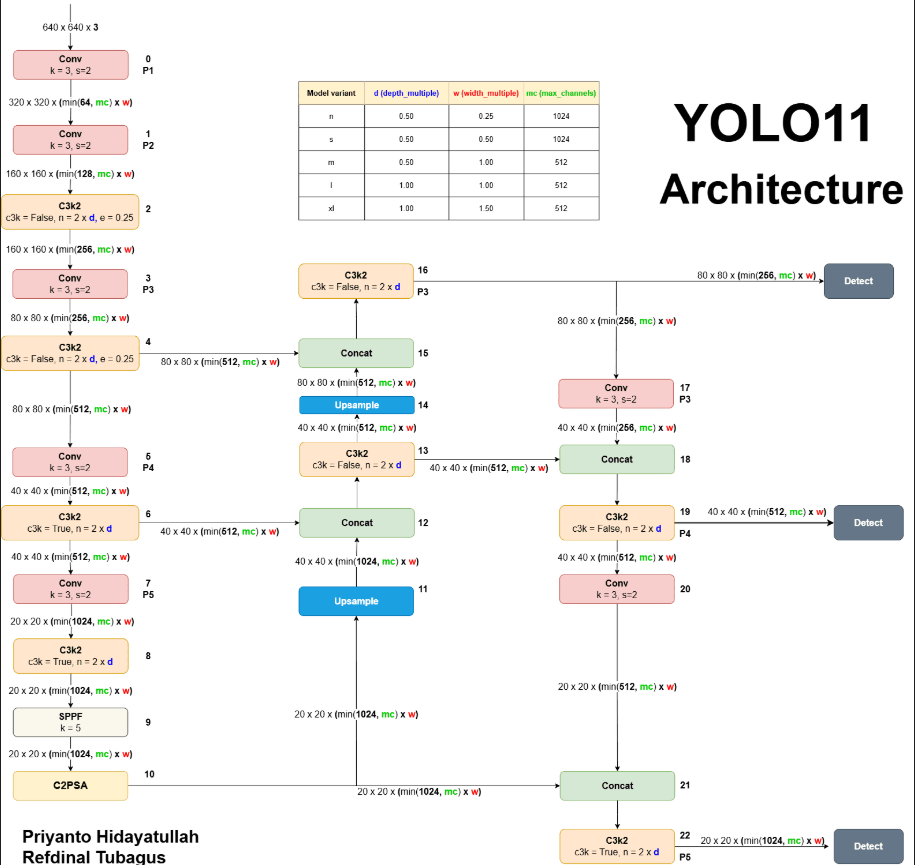
\includegraphics[width=\textwidth]{imgs/yolo11-architecture}
    \caption{YOLOv8 网络结构示意图}
    \label{图1:}
\end{figure}

\subsection{Faster R-CNN}
Faster R-CNN是两阶段检测器的代表,由Ren等人于2015年提出。
它通过引入区域候选网络(Region Proposal Network, RPN)实现了端到端的训练,极大地提升了检测速度。
RPN是一个全卷积网络,用于预测目标边界框和目标得分,从而生成高质量的候选区域。
RoI Pooling将不同大小的候选区域映射到固定大小的特征图上,以便后续的全连接层进行分类和回归。
图2描述了Faster R-CNN的网络架构图。
\begin{figure}[h!]
    \centering
    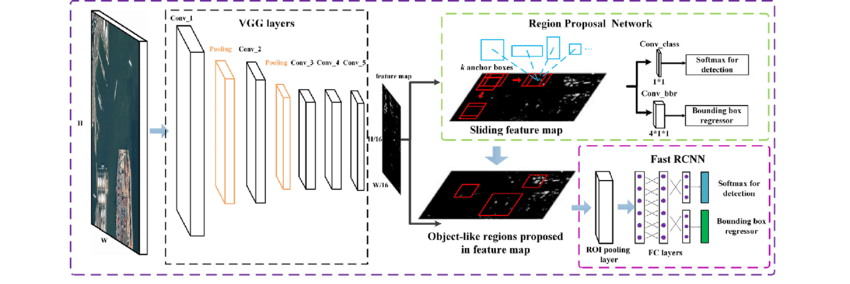
\includegraphics[width=\textwidth]{imgs/The-architecture-of-Faster-R-CNN}
    \caption{Faster R-CNN 网络结构示意图}
    \label{图2:}
\end{figure}

\section{实验目的:}
\begin{enumerate}
    \item 熟悉并掌握至少3-5种主流目标检测算法(如YOLO系列、Faster R-CNN、FCOS等)的基本原理和应用。
    \item 学习如何在Python环境中部署和调用开源目标检测项目的API。
    \item 实现对校园内自行拍摄图像的目标检测,并对检测结果进行验证和分析。
\end{enumerate}


\section{实验内容:}
调用开源的目标检测算法(YOLO, Faster RCNN, FCOS等)的API,实现目标检测
可自行选择自己感兴趣的3-5个目标检测算法,部署其开源项目,使用校园内自行拍摄的多个图像进行目标检测结果验证和分析。


% \section{实验器材(设备、元器件):}
% \subsection{硬件环境}
\begin{itemize}
    \item \textbf{处理器 (CPU)}: Intel Core i7-XXXX / AMD Ryzen X XXXX 或更高
    \item \textbf{图形处理器 (GPU)}: NVIDIA GeForce RTX 30XX / 40XX 系列或同等性能的GPU,推荐显存不低于8GB,用于加速深度学习模型的推理。
    \item \textbf{内存 (RAM)}: 16GB 或更高
    \item \textbf{存储}:500GB SSD 或更大,用于存储数据集、模型权重和代码。
\end{itemize}

\subsection{软件环境}
\begin{itemize}
    \item \textbf{操作系统}: Windows 10/11, Ubuntu 18.04/20.04 LTS
    \item \textbf{编程语言}: Python 3.8+
    \item \textbf{深度学习框架}: PyTorch 1.8+ 或 TensorFlow 2.x
    \item \textbf{Python 包管理}: pip 或 conda
    \item \textbf{集成开发环境 (IDE)}: Visual Studio Code 或 PyCharm
    \item \textbf{版本控制}: Git
\end{itemize}

\subsection{主要库和依赖}
\begin{itemize}
    \item \textbf{PyTorch/TensorFlow}: 深度学习核心框架。
    \item \textbf{torchvision/tensorflow-addons}: 图像处理和计算机视觉相关工具。
    \item \textbf{OpenCV-Python}: 图像处理库,用于图像的读取、显示和预处理。
    \item \textbf{Numpy}: 科学计算库。
    \item \textbf{Matplotlib/Pillow}: 用于结果可视化。
    \item \textbf{mmcv-full}: OpenMMLab系列算法(如MMDetection)的通用视觉库。
    \item \textbf{ultralytics}: YOLOv8等Ultralytics系列模型的官方库。
\end{itemize}

\subsection{实验数据集}
\begin{itemize}
    \item \textbf{校园图像数据集}: 自行拍摄的校园内图像,包含多种场景和目标,如教学楼、图书馆、宿舍、食堂、道路、绿化带、行人、自行车、汽车等。图像数量建议在20-50张之间,分辨率不低于1920x1080。
\end{itemize}
\todo{校园图像数据集示例}


\section{实验步骤:}
\subsection{开源项目部署与模型下载}
从GitHub克隆所选算法的官方开源项目到本地。
进入每个项目的根目录,根据其`requirements.txt`或`setup.py`安装特有的依赖库。
从官方提供的模型库下载对应算法的预训练权重文件。
例如,YOLOv8的`yolov8n.pt`,MMDetection中Faster R-CNN或FCOS的`.pth`文件。

\subsection{图像数据准备}
在不同校园内不同地点、不同光照条件下拍摄多张图像,
地点包括办公室,食堂,教室等,
时间主要包括上午和晚上的情况以模拟不同情况下的光照条件。
将所有拍摄的图像统一存放在一个新建的文件夹中。

\subsection{目标检测API调用与结果获取}
针对每种选定的算法,查阅模型的官方文档,
编写独立的Python模块,用于加载模型、读取图像、执行推理并获取检测结果。
将每张图像的检测结果直接在图像上绘制的方式保存。

\subsection{结果可视化与分析}
在detectionAPIs.ipynb笔记本上开辟独立的单元格,
执行上一步写好的API调用函数,
分别查看不同算法在相同图像上的检测效果,
定性观察其在目标识别准确性、定位精度、小目标检测、密集目标处理、抗遮挡能力等方面的表现。

\section{实验数据及结果分析:}
我们选取的校园场景图片如图1所示。
\begin{figure}[h!]
    \centering
    \includegraphics[width=\textwidth]{imgs/origin.png}
    \caption{原始校园场景图片}
    \label{fig:origin_image}
\end{figure}

\subsubsection{MMDetection 检测结果}
我们利用MMDetection的API工具,检测到的结果如图2所示。

\begin{figure}[h!]
    \centering
    \includegraphics[width=\textwidth]{imgs/mmdetection.png}
    \caption{FCOS 检测结果示意图}
    \label{fig:fcos_result}
\end{figure}


\subsubsection{YOLOv8 检测结果}
我们利用MMDetection的API工具,检测到的结果如图3所示。

\begin{figure}[h!]
    \centering
    \includegraphics[width=\textwidth]{imgs/yolo.png}
    \caption{YOLOv8 检测结果示意图}
    \label{fig:yolov8_result}
\end{figure}

\subsubsection{Faster R-CNN 检测结果}
由于此API没有可视化较好的工具,
因此选择一张样例图片,这是上述场景图片的第四张。
输出检测出的bbox坐标,结果如图4所示。

\begin{figure}[h!]
    \centering
    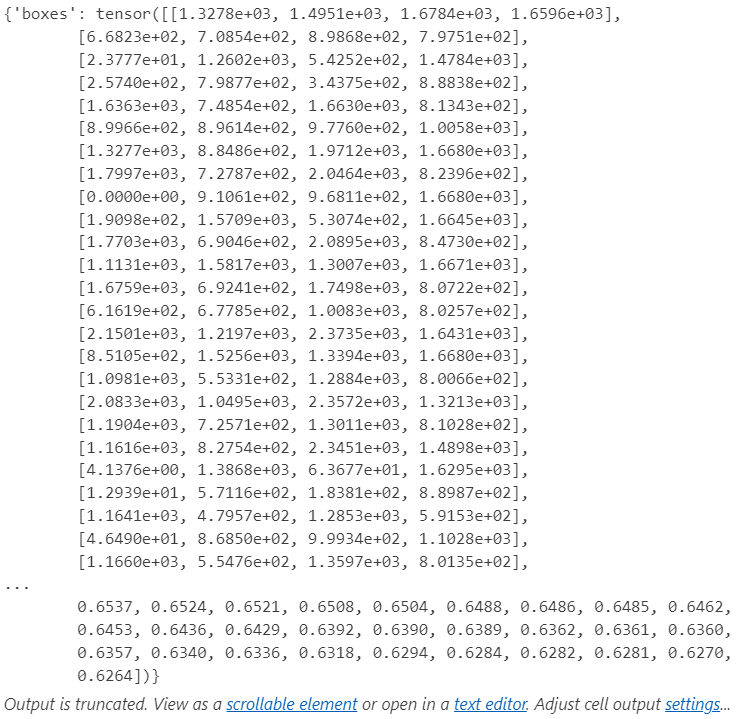
\includegraphics[width=\textwidth]{imgs/fast_res.png}
    \caption{Faster R-CNN 检测结果示意图}
    \label{fig:fasterrcnn_result}
\end{figure}




\section{实验结论:}
\begin{enumerate}
    \item 检测准确性: 可以看到YOLO模型效果比MMDetection效果更好,能检测的物体位置更准确。
    \item 定位精度: 可以看到YOLO在观察小目标、密集目标和遮挡情况下的定位更好。
    \item 误检与漏检: MMDetection漏检情况较多,但两个模型基本都没有错检的情况。
\end{enumerate}


\section{总结及心得体会:}
尽管实验成功验证了核心原理并构建了基本框架,但也认识到当前实现作为生产级编译器前端存在诸多不足(如错误恢复的健壮性、符号表中信息的完整性、对复杂文法结构的处理能力、性能优化以及与现代编译器架构的差距等)。

总而言之,本次实验通过从零开始实现一个简单的编译器前端,不仅成功地将编译原理的理论知识转化为实际代码。 通过构建了一个可工作的简单demo,我加深了对词法分析、语法分析、作用域管理和符号表工作原理的理解。实验结果证明了所采用方法的有效性。

\section{对本实验过程及方法的改进建议:}
错误恢复机制 :本项目的词法分析器在遇到非法字符或错误时,会跳过当前行的剩余部分并返回错误。这是一种简单的恐慌模式错误恢复策略,即在检测到错误后,跳过一部分输入直到找到一个看似可以继续解析的同步点。可以设计更加用户友好的错误报告,比如“在 X 处期望得到 Y,但找到了 Z”,并给出可能的修正建议。还比如不仅仅跳到行尾,而是跳到更合适的同步词法单元,例如语句结束符 ;、块的开始/结束符号 (begin, end) 或文件末尾。这需要在文法中定义哪些词法单元可以作为同步点。

目前,对于变量声明的情况,无法维护其所属的过程名。在支持嵌套函数或过程的语言中,一个变量的完全限定名或用于查找作用域链的信息通常需要包含其所在的函数/过程信息。 在解析函数体或任何可能包含变量声明的块时,可以将当前正在解析的函数/过程的名称作为参数传递给其他方法,限于时间有限无法完成。

在文法中没有区分实参和形参,导致进一步语义分析可能出现了意料不到的错误。函数定义时的参数列表(形参)应该在函数体的局部作用域内进行声明,并且这些形参应该在函数体内部可见。这可能需要修改文法来明确区分函数定义和函数调用,并为函数定义引入形参列表的文法规则,例如 <形参列表> → <变量> { , <变量> } | ε

我们只对文件流进行了简化实现,在prep.rs 中的文件不足可能在于错误处理比较简单,以及没有考虑字符编码问题。lex.rs 和 parse.rs 中的文件错误输出每次都会新建并覆盖文件,没有追加功能。而且错误应该输出到标准错误流而不是标准输出,这在命令行工具中是更好的实践。应该采用更安全的IO方式;

lex.rs 中的 current_token 方法是手写的状态转换逻辑,模拟了有限自动机。
手写 DFA 对于简单文法是可行的,但对于复杂语言,状态和转换会变得非常多且难以管理,容易出错。之后可以尝试手动实现一个表驱动的 DFA,根据当前状态和输入字符查找下一个状态。

输入优化:Lexer 在 getchar 中使用下标索引的来获取字符。这种方式在 pos 较大时效率较低,因为它需要从字符串的开头开始遍历字符直到 pos 位置.更好的方式是使用 
缓冲读取,对于非常大的文件,可以考虑实现或使用带缓冲的文件读取,而不是一次性将整个文件读入内存。


\vspace{4cm}
\begin{flushright}
\begin{tabular}{lc}
\sihao{\hei{报告评分:}}& \sihao{\song{~~~~~~}}\\
\sihao{\hei{指导教师签字:}}& \sihao{\song{~~~~~~}}\\
\end{tabular}
\end{flushright}

\newpage

\begin{appendix}
\section{代码示例}

如代码1, 2,3 所示,分为三个部分mmdet.py, yolo.py, fastrcnn.py

\begin{lstlisting}[caption={mmdet.py}, label={lst:code-example}, captionpos=t, language=python]
    from mmdet.registry import VISUALIZERS
    import mmcv
    from mmdet.apis import init_detector, inference_detector
    import cv2

    # init the visualizer(execute this block only once)
    config_file = '../data/mmdet/rtmdet_tiny_8xb32-300e_coco.py'
    checkpoint_file = '../data/mmdet/rtmdet_tiny_8xb32-300e_coco_20220902_112414-78e30dcc.pth'
    model = init_detector(config_file, checkpoint_file, device='cpu')  # or device='cuda:0'
    visualizer = VISUALIZERS.build(model.cfg.visualizer)
    # the dataset_meta is loaded from the checkpoint and
    # then pass to the model in init_detector
    visualizer.dataset_meta = model.dataset_meta

    # show the results
    for i in range(4):
        img = mmcv.imread(f'../data/{i}.jpg', channel_order='rgb')
        result = inference_detector(model, img)
        visualizer.add_datasample(
            'result',
            img,
            data_sample=result,
            draw_gt=False,
            wait_time=0,
        )
        visualizer.show()
        visualized_img = visualizer.get_image()
        cv2.imwrite(f'../data/mmdet/{i}_result.jpg', visualized_img)
\end{lstlisting}

\begin{lstlisting}[caption={yolo.py}, label={lst:code-example}, captionpos=t, language=python]
    from ultralytics import YOLO

    # Create a new YOLO model from scratch
    model = YOLO("yolo11.yaml")

    # Load a pretrained YOLO model (recommended for training)
    model = YOLO("yolo11n.pt")

    # Train the model using the 'coco8.yaml' dataset for 3 epochs
    results = model.train(data="coco8.yaml", epochs=3)

    # Evaluate the model's performance on the validation set
    results = model.val()

    # Perform object detection on an image using the model
    for i in range(4):
        results = model(f"../data/{i}.jpg")
        results[0].save(f'../data/yolo/{i}_result.jpg')

    # Export the model to ONNX format
    success = model.export(format="onnx")
\end{lstlisting}

\begin{lstlisting}[caption={fastrcnn.py}, label={lst:code-example}, captionpos=t, language=python]
    import torch
    import torchvision
    from torchvision.models.detection import FasterRCNN_ResNet50_FPN_Weights
    from torchvision.models.detection.faster_rcnn import FastRCNNPredictor
    from torchvision.transforms import functional as F
    from PIL import Image

    weights = FasterRCNN_ResNet50_FPN_Weights.DEFAULT 
    model = torchvision.models.detection.fasterrcnn_resnet50_fpn(weights=weights)

    print(model)
    num_classes = 2 
    in_features = model.roi_heads.box_predictor.cls_score.in_features
    model.roi_heads.box_predictor = FastRCNNPredictor(in_features, num_classes)
    model.eval()
    dummy_image = torch.rand(1, 3, 800, 800)

    img_path = "../data/3.jpg"
    img = Image.open(img_path).convert("RGB")
    preprocess = weights.transforms()
    image_tensor = preprocess(img).unsqueeze(0) # Add batch dimension

    with torch.no_grad(): 
        predictions = model(image_tensor) 
        print(predictions[0])
\end{lstlisting}
\end{appendix}

\end{document}
